\documentclass[a4paper,11pt]{article}
\usepackage{amsmath,amsthm,amsfonts,amssymb,amscd,amstext,vmargin,graphics,graphicx,tabularx,multicol} 
\usepackage[francais]{babel}
\usepackage[utf8]{inputenc}  
\usepackage[T1]{fontenc} 
\usepackage{pstricks-add,tikz,tkz-tab,variations}
\usepackage[autolanguage,np]{numprint} 

\setmarginsrb{1.5cm}{0.5cm}{1cm}{0.5cm}{0cm}{0cm}{0cm}{0cm} %Gauche, haut, droite, haut
\newcounter{numexo}
\newcommand{\exo}[1]{\stepcounter{numexo}\noindent{\bf Exercice~\thenumexo} : \marginpar{\hfill /#1}}
\reversemarginpar


\newcounter{enumtabi}
\newcounter{enumtaba}
\newcommand{\q}{\stepcounter{enumtabi} \theenumtabi.  }
\newcommand{\qa}{\stepcounter{enumtaba} (\alph{enumtaba}) }
\newcommand{\initq}{\setcounter{enumtabi}{0}}
\newcommand{\initqa}{\setcounter{enumtaba}{0}}

\newcommand{\be}{\begin{enumerate}}
\newcommand{\ee}{\end{enumerate}}
\newcommand{\bi}{\begin{itemize}}
\newcommand{\ei}{\end{itemize}}
\newcommand{\bp}{\begin{pspicture*}}
\newcommand{\ep}{\end{pspicture*}}
\newcommand{\bt}{\begin{tabular}}
\newcommand{\et}{\end{tabular}}
\renewcommand{\tabularxcolumn}[1]{>{\centering}m{#1}} %(colonne m{} centrée, au lieu de p par défault) 
\newcommand{\tnl}{\tabularnewline}

\newcommand{\bmul}[1]{\begin{multicols}{#1}}
\newcommand{\emul}{\end{multicols}}

\newcommand{\trait}{\noindent \rule{\linewidth}{0.2mm}}
\newcommand{\hs}[1]{\hspace{#1}}
\newcommand{\vs}[1]{\vspace{#1}}

\newcommand{\N}{\mathbb{N}}
\newcommand{\Z}{\mathbb{Z}}
\newcommand{\R}{\mathbb{R}}
\newcommand{\C}{\mathbb{C}}
\newcommand{\Dcal}{\mathcal{D}}
\newcommand{\Ccal}{\mathcal{C}}
\newcommand{\mc}{\mathcal}

\newcommand{\vect}[1]{\overrightarrow{#1}}
\newcommand{\ds}{\displaystyle}
\newcommand{\eq}{\quad \Leftrightarrow \quad}
\newcommand{\vecti}{\vec{\imath}}
\newcommand{\vectj}{\vec{\jmath}}
\newcommand{\Oij}{(O;\vec{\imath}, \vec{\jmath})}
\newcommand{\OIJ}{(O;I,J)}


\newcommand{\reponse}[1][1]{%
\multido{}{#1}{\makebox[\linewidth]{\rule[0pt]{0pt}{20pt}\dotfill}
}}

\newcommand{\titre}[5] 
% #1: titre #2: haut gauche #3: bas gauche #4: haut droite #5: bas droite
{
\noindent #2 \hfill #4 \\
#3 \hfill #5

\vspace{-1.6cm}

\begin{center}\rule{6cm}{0.5mm}\end{center}
\vspace{0.2cm}
\begin{center}{\large{\textbf{#1}}}\end{center}
\begin{center}\rule{6cm}{0.5mm}\end{center}
}



\begin{document}
\pagestyle{empty}
\titre{Interrogation: Section d'une solide par un plan}{Nom :}{Prénom :}{Classe}{Date}

\begin{flushleft}
\begin{tabular}{|m{9.5cm}|m{1.25cm}|m{1.25cm}|m{1.25cm}|m{1.25cm}|m{1.25cm}|}
\hline 
\textbf{Compétences} & \begin{center}
\textbf{N.E.}
\end{center} & \begin{center}
\textbf{M.I.}
\end{center} & \begin{center}
\textbf{M.F.}
\end{center}  & \begin{center}
\textbf{M.S.}
\end{center} & \begin{center}
\textbf{T.B.M.}
\end{center} \\ 
\hline 
Je dois savoir analyser et étudier les sections de certains solides par un plan &  &  & & &\\
\hline 
Je dois savoir construire en vraie grandeur les sections de certains solides par un plan &  &  & & &\\
\hline
Je dois savoir utiliser, produire et mettre en relation des situations spatiales (schémas, croquis, maquettes, patrons, coordonnées dans l'espace, différents théorèmes) &  &  & & &\\ 
\hline


\end{tabular} 
\end{flushleft}

\textit{N.E = Non évalué ; M.I. = Maîtrise insuffisante ; M.F. = Maîtrise fragile ; M.S. = Maîtrise satisfaisante ; T.B.M. = Très bonne maîtrise}\\


\vspace*{0.5cm}

\exo{1.5} Dans chaque cas, tracer la section du solide par le plan (IJK) ou tracer la section du solide avec le plan parallèle à la face hachurée passant par I.

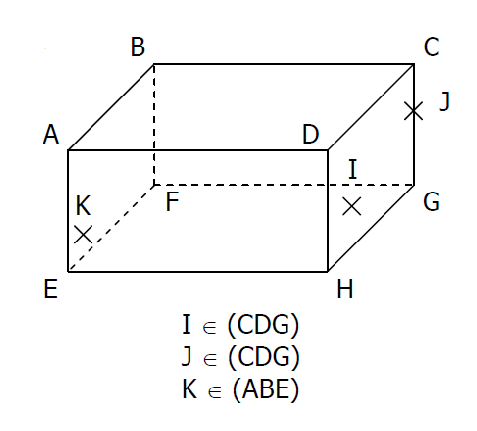
\includegraphics[scale=0.85]{interro1.eps}  \includegraphics[scale=0.9]{interro2.eps}  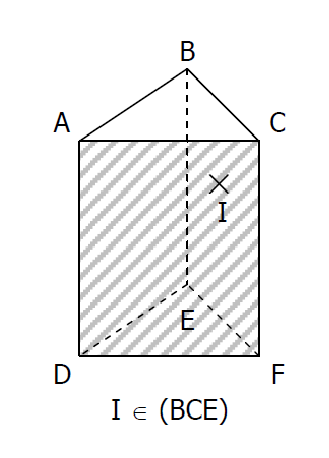
\includegraphics[scale=1]{interro3.eps} \\


\exo{2.5} Soient ABCDEFGH est un pavé droit et le point K, le centre du pavé droit. On considère le repère (A ; [AB) ;
[AD) ; [AE)).\\

\bmul{2}

\begin{flushleft}
\includegraphics[scale=0.85]{interro4.eps} 
\end{flushleft}

\columnbreak

\q Donner les coordonnées des points B, E, C et K.\\
\reponse[3]\\

\q Placer les points suivants :\\

 S(4 ; 3 ; 1) ; R(0 ; 7 ; 3) et M(9 ; 8 ; 2) \\


\emul
\newpage

\exo{3} 

\bmul{2}

ABCDEFGH est un pavé droit que l'on a coupé par un plan parallèle à l’arête [GH]. Les dimensions sont indiquées sur la figure.

\textbf{\underline{Étude de la section}}



\columnbreak

\includegraphics[scale=0.85]{interro5.eps} 

\emul

\initq \q Quelle est la nature de cette section ? Justifier votre réponse.\\
\reponse[3]\\

\q Dessiner cette section en vraie grandeur. Si besoin, justifier votre réponse.\\


\vspace*{4cm}

\textbf{\underline{Étude du solide DHICGJ obtenu}}\\

\initq \q Quelle est la nature du solide DHICGJ ? Aucune justification n'est attendue.\\
 \reponse[1]\\

\q Calculer le volume de ce solide.\\
\reponse[4]\\

\vspace*{0.3cm}

\exo{3} On considère un cylindre de révolution de hauteur 7 cm et dont le disque de base à un rayon de 4 cm. \\

\bmul{2}

 On coupe ce cylindre par un plan parallèle à son axe et qui coupe un rayon du disque de base à 2 cm de son centre.\\

\initq \q Quelle est la nature de la section du cylindre par ce plan ?  Justifier votre réponse.\\
\reponse[4]

\columnbreak

\bmul{2}


\includegraphics[scale=0.85]{interro6.eps}

\columnbreak

 Agrandissement du disque supérieur du cylindre\\
 \includegraphics[scale=0.7]{interro7.eps} 
 
 \emul

\emul

\newpage

\vspace*{0.2cm}

\q Pour trouver les dimensions de cette section on travaille dans le disque de base dans lequel on souhaite trouver la longueur AC.\\



\qa Préciser, sans justifier, les longueurs OC et OB.\\
\reponse[2]\\

\qa Calculer la longueur BC. Et en déduire la longueur AC.\\
\reponse[7]\\

\qa Représenter en vraie grandeur la section du cylindre avec ce plan. 

\end{document}
